\documentclass[tikz,border=3pt]{standalone}
\usetikzlibrary{arrows.meta}
\begin{document}
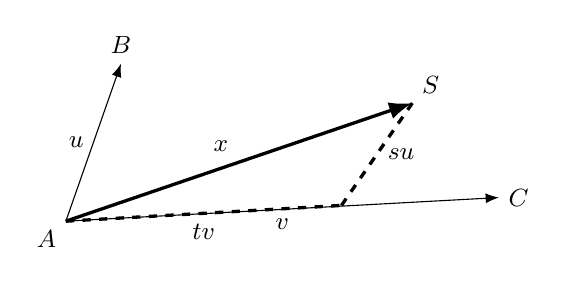
\begin{tikzpicture}[>=Latex, font=\small]
  \coordinate (A) at (0,0);
  \coordinate (B) at (0.7,2.0);
  \coordinate (C) at (5.5,0.3);
  \coordinate (TV) at (3.5,0.2);
  \coordinate (S) at (4.4,1.5);

  \draw[->] (A) -- (C) node[midway, below] {$v$} node[right] {$C$};
  \draw[->] (A) -- (B) node[midway, left] {$u$} node[above] {$B$};

  \draw[dashed, very thick] (A) -- (TV) node[midway, below] {$tv$};
  \draw[dashed, very thick] (TV) -- (S) node[midway, right] {$su$};
  \draw[->, very thick] (A) -- (S) node[midway, above left] {$x$};

  \node[below left] at (A) {$A$};
  \node[above right] at (S) {$S$};
\end{tikzpicture}
\end{document}
